\section{Flujo de trabajo}
\label{ch:propuesta:sec:flujoDeTrabajo}

Actualmente existen flujos de trabajo para la extracción de supeficies \cite{Ruprecht94ascheme}\cite{Dietrich_marchingcubes}, los cuales intentan generar superficies sin los principales problemas topológicos explicados en \ref{subsec:marchingCubes:consecuencias}. El flujo de trabajo propuesto en esta investigación se muestra en la fugura \ref{f:flujoDeTrabajo:flujoDeTrabajo}

\begin{figure}[htb]
\centering
	\includegraphics[width=0.5\textwidth]{images/misc/workflow.pdf}
\caption{Flujo de trabajo propuesto}
\label{f:flujoDeTrabajo:flujoDeTrabajo}
\end{figure}

Cada uno de estos pasos serán explicados a continuación.
\newpage

\subsection{Extracción de datos}
\label{ch:propuesta:sec:extraccionDeDatos}

En primera instancia, para extraer una superficie desde una nube de puntos, es necesario recolectar estos puntos, para eso existen diversas técnicas y propósitos. Para el propósito de esta investigación, el formato de los datos debe ser un \emph{dataset} de imágenes coaxiales que individualmente muestran una seccion planar de la superficie que se quiere extraer, y en conjunto describen la superficie completa.

\subsubsection{Imágenes por resonancia magnética}
\label{ch:propuesta:sec:extraccionDeDatos:subsec:imagenesPorResonanciaMagnetica}

En el análisis de imágenes médicas, en ocaciones se necesita visualizar \emph{datasets} volumétricos, cortes en tres dimensiones de los órganos que se quieren estudiar, como las imágenes obtenidas por resonancia magnética (\emph{MRI}, de sus siglas en inglés \emph{Magnetic resonance imaging}).

Las imágenes por resonancia magnética son una técnica de imagenología usada principalmente en el área médica para producir imágenes de alta calidad del interior del cuerpo humano. Estas imágenes son basadas en el principio de la resonancia nuclear magnética, una técnica espectroscópica usada por científicos para obtener información física y química acerca de las moléculas. Ya en el año 2003 existían aproximadamente mas de diez mil unidades de resonancia magnética y aproximadamente setenta y cinco millones de exámenes realizados por año \footnote{Joseph P. Hornak, Ph.D. \textit{The Basics of MRI}, http://www.cis.rit.edu/htbooks/mri/ (19 sept. 2012).}

Las imágenes obtenidas de estos exámenes pueden ser pensadas como imágenes en tres dimensiones donde cada \emph{pixel} (o \emph{voxel}, elemento de volúmen) representa una cantidad medible de volumen en alguna posición $(x, y, z)$ del espacio. Un ejemplo de estas imágenes se muestra en la figura \ref{f:flujoDeTrabajo:mri_joe} \footnote{MRI, CPO Abdomen Total, paciente Joe Cabezas Campos, estudio 040501000, Integramedica, Av. Libertador Bernardo O'Higgins 1620, 26 junio 2012 19:35}

\begin{figure}[p]
\centering
	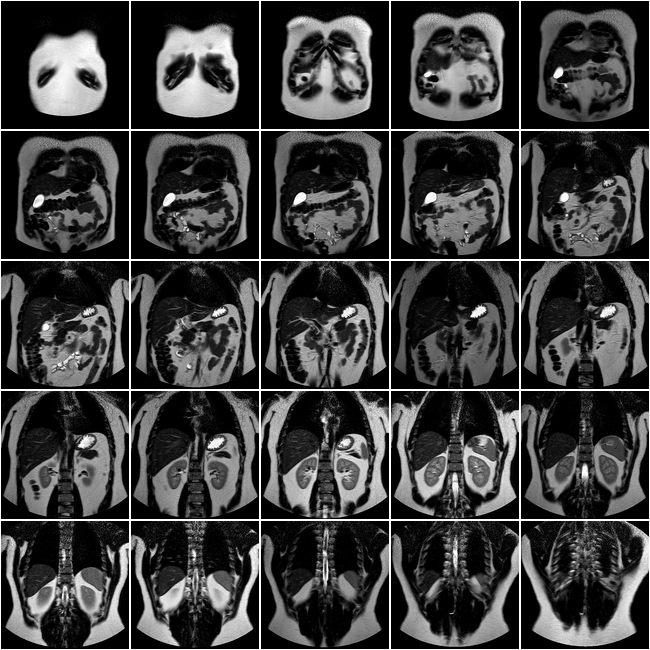
\includegraphics[width=1.0\textwidth]{images/misc/mri_joe.png}
\caption{Un \emph{dataset} de 28 imágenes de un examen de resonancia magnética}
\label{f:flujoDeTrabajo:mri_joe}
\end{figure}

Una forma de visualizar el cuerpo en tres dimensiones es extrayendo una \emph{isosuperficie} usando el algoritmo de \emph{Marching Cubes}.

En esta investigación, la totalidad de los dataset usados para la implementación del algoritmo de \emph{Marching Cubes} son extraidos de imágenes de resonancia magnética.
\newpage

\subsubsection{Funciones en tres dimensiones}
\label{ch:propuesta:sec:extraccionDeDatos:subsec:funcionesEnTresDimensiones}

